% Метод управления трафиком в гибридной программно-определяемой сети
\section{Распрацоўка праграмнага забеспячэння для кіравання трафікам ў гібрыдных сетках SDN}

На аснове вышэй апісаных вывадаў разгледзем гібрыдную мадэль SDN
пабудаваную ў сетцы з пратаколам маршрутызацыі EIGRP.

\subsection{Прынцып работы пратакола EIGRP}

EIGRP (англ. Enhanced Interior Gateway Routing Protocol) --- пратакол маршрутызацыі, распрацаваны фірмай Cisco на аснове пратаколу IGRP той жа фірмы. Рэліз пратаколу адбыўся ў 1994 годзе. EIGRP выкарыстоўвае механізм DUAL (diffusing update algorithm) для выбару найбольш кароткага маршруту.

EIGRP больш просты ў рэалізацыі і меней патрабавальны да вылічальных рэсурсаў маршрутызатара чым пратакол OSPF (Open Shortest Path First). Таксама EIGRP мае больш удасканалены алгарытм вылічэння метрыкі (DUAL), які можа выкарыстоўваць 5 розных кампанентаў для разліку:

\begin{enumerate}
    \item прапускная здольнасць (Bandwidth) --- мінімальная прапускная здольнасць для дадзенага маршруту (а не сума коштаў (cost) у адрозненне ад OSPF).
    \item Затрымка (Delay) --- cумарная затрымка на ўсім шляху маршруту.
    \item Надзейнасць (Reliability) --- найгоршы паказчык надзейнасці на ўсім шляху маршруту, заснаваны на характарыстыкі keep alive.
    \item Нагрузка (Loading) --- найгоршы паказальнік нагрузкі інтэрфейса на ўсім шляху маршруту, заснаваны на колькасці трафіку, які праходзіць праз інтэрфейс і параметры bandwidth на гэтым інтэрфейсе.
    \item MTU (Maximum transmission unit) --- мінімальны памер MTU на ўсім шляху маршруту.
\end{enumerate}

Па ўмаўчанні, EIGRP выкарыстоўвае толькі першыя два кампаненты, так як надзейнасць і нагрузка --- дынамічныя велічыні, якія могуць змяняцца да некалькіх раз у секунду. Адпаведна, кожнае змяненне выклікае пераразлік метрыкі для маршрутаў і выкарыстанне працэсарнай магутнасці маршрутызатара да 100\%. MTU не з'яўляецца дынамічнай велічынёй, але не выкарыстоўваецца па прычыне слабога ўплыву на метрыку маршруту.

Асноўныя характарыстыкі EIGRP:
\begin{enumerate}
     \item хуткая збежнасць (у параўнанні з іншымі дыстанцыйна-вектарнымі пратаколамі);
     \item падтрымка VLSM (Variable Length Subnet Masking);
     \item частковыя абнаўлення паміж суседзямі;
     \item падтрымка розных пратаколаў сеткавага ўзроўня (IP, IPX, AppleTalk);
     \item аднолькавыя настройкі пратакола пры выкарыстанні розных пратаколаў канального ўзроўню (напрыклад, у OSPF настройкі адрозніваюцца для Ethernet і Frame Relay);
     \item складаная метрыка;
     \item выкарыстанне multicast (224.0.0.10) і unicast адрасоў, замест шырокавяшчальнай рассылкі;
\end{enumerate}

\subsubsection{RTP і тыпы паведамленняў EIGRP.}

RTP (Reliable Transport Protocol) кіруе працэсам адпраўкі і атрымання пакетаў EIGRP.

RTP забяспечвае:
\begin{enumerate}
    \item гарантаваную дастаўку пакетаў. Для гэтага выкарыстоўваецца прапрыетарны алгарытм Cisco, reliable multicast. Пакеты адпраўляюцца на multicast-адрас 224.0.0.10. Кожны сусед які атрымаў такі пакет адпраўляе пацверджанне адпраўніку пакета.
    \item захаванне парадку пакетаў. У кожным пакеце выкарыстоўваецца два нумары паслядоўнасці (sequence). Кожны пакет уключае ў сябе нумар прысвоены яму адпраўніком. Гэты нумар павялічваецца на адзінку кожны раз, калі маршрутызатар адпраўляе новы пакет. Акрамя таго, адпраўнік змяшчае ў пакет нумар апошняга атрыманага пакета ад атрымальніка.
    \item у некаторых выпадках RTP выкарыстоўвае негарантаваную дастаўку. У такіх пакетах нe прастаўляюцца нумары паслядоўнасці і яны не патрабуюць пацвярджэння аб атрыманнi.
\end{enumerate}

Усе паведамленні EIGRP інкапсулюецца ў IP-пакеты, нумар EIGRP ў полі пратакол IP-пакета --- 88.

EIGRP выкарыстоўвае 5 тыпаў паведамленняў:
\begin{enumerate}
    \item Hello --- маршрутызатары выкарыстоўваюць hello-пакеты для выяўлення суседзяў. Пакеты адпраўляюцца пры дапамозе multicast рассылкі і не патрабуюць пацвярджэння аб атрыманнi;
    \item Update --- змяшчаецца інфармацыя аб змене маршрутаў. Яны адпраўляюцца толькі маршрутызатарам, якіх тычыцца абнаўленне. Гэтыя пакеты могуць быць адпраўленыя канкрэтнаму маршрутызатару (unicast рассылка) або групе маршрутызатараў (multicast рассылка). Атрыманне update-пакета пацвярджаецца адпраўкай ACK пакета;
    \item Query --- калі маршрутызатар выконвае падлік маршруту і ў яго няма feasible successor, ён адпраўляе query-пакет сваім суседзям для таго каб вызначыць ці няма feasible successor для гэтага маршруту ў іх. Звычайна query-пакеты адпраўляюцца multicast рассылкай, але могуць быць і unicast рассылкай. Атрыманне query-пакета пацвярджаецца адпраўкай ACK атрымальнікам пакета;
    \item Reply --- маршрутызатар адпраўляе reply-пакет у адказ на query-пакет. Reply-пакеты адпраўляюцца unicast рассылкай таму, хто адправіў query-пакет. Атрыманне reply-пакета пацвярджаецца адпраўкай ACK;
    \item ACK --- пакет, які пацвярджае атрыманне пакетаў update, query, reply. ACK-пакеты адпраўляюцца unicast рассылкай і ўтрымліваюць у сабе acknowledgment number. Фактычна гэта hello-пакеты, якія не перадаюць даных. Выкарыстоўваецца негарантаваная дастаўка.
\end{enumerate}

\subsubsection{Адносіны суседства і пакеты Hello.}

Для ўстанаўлення адносін суседства EIGRP выкарыстоўвае пакеты hello:
\begin{enumerate}
    \item на ethernet-інтэрфейсах і point-to-point інтэрфейсах hello-пакеты па ўмаўчанні адпраўляюцца кожныя 5 секунд, але з невялікім выпадковым адхіленнем, якое выкарыстоўваецца для таго, каб паміж маршрутызатарамі не было сінхранізацыі ў адпраўцы hello-пакетаў;
    \item на multipoint X.25, Frame Relay, і ATM інтэрфейсах hello-пакеты адпраўляюцца unicast па змаўчанні кожныя 60 секунд;
    \item калі сусед не дасылае hello-паведамленне за перыяд hold time (па ўмаўчанні 15 секунд, 3 hello-інтэрвалы), то ён лічыцца недаступным.
\end{enumerate}

Для таго каб маршрутызатары сталі суседзямі павінны выконвацца такія ўмовы:
\begin{enumerate}
    \item маршрутызатары павінны прайсці аўтэнтыфікацыю;
    \item маршрутызатары павінны быць у адной AS (Autonomous System);
    \item адносіны суседства павінны ўстанаўлівацца на галоўных адрасах (калі прыходзіць hello-пакет, маршрутызатар правярае ці належыць адрас адпраўніка сетцы на галоўным адрасе інтэрфейса);
    \item павінны супадаць значэння K-каэфіцыентаў.
\end{enumerate}

Інфармацыя аб усіх выяўленых суседзях змяшчаецца ў табліцы суседзяў.
Табліца суседзяў (neighbor table) --- спіс непасрэдна далучаных маршрутызатараў (на якіх працуе EIGRP) з якімі маршрутызатар устанавіў адносіны суседства. Адна табліца суседзяў існуе для кожнага PDM (Protocol-dependent module).

\subsubsection{Update пакеты.}

Пасля таго як маршрутызатары сталі суседзямі, яны пачынаюць абменьвацца абнаўленнямі (Update). Гэтыя пакеты могуць быць адпраўленыя канкрэтнаму маршрутызатара (unicast рассылка) або групе маршрутызатараў (multicast рассылка).

Працэс абмену абнаўленнямі:
\begin{enumerate}
    \item першапачаткова адпраўляюцца поўныя абнаўлення, у якія ўключаны ўсе маршруты, за выключэннем тых, якія трапляюць пад правіла split horizon;
    \item пасля таго як абмен маршрутамі завяршыўся, абнаўленні не адпраўляюцца;
    \item у далейшым абнаўлення адпраўляюцца, калі змяніўся адзін або больш маршрутаў;
    \item калі адносіны суседства разрываюцца, а затым аднаўляюцца, то адпраўляюцца поўныя абнаўлення.
\end{enumerate}

Віды EIGRP абнаўленняў:
\begin{enumerate}
    \item неперыядычныя (Nonperiodic) --- абнаўленні адпраўляюцца нe праз рэгулярныя інтэрвалы часу, а пры змене тапалогіі або метрыкі;
    \item частковыя (Partial) --- у абнаўленнях перадаецца не ўся інфармацыя з табліцы маршрутызацыі, а толькі змены;
    \item абмежаваныя (Bounded) - абнаўленні адпраўляюцца толькі задзейнічаным маршрутызатарам.
\end{enumerate}

\subsubsection{Табліца тапалогіі}

Табліца тапалогіі (topology table) --- спіс маршрутаў, вывучаных ад кожнага суседа.

Калі сусед паведамляе лакальнаму маршрутызатару аб маршруце, то сусед павінен выкарыстоўваць гэты маршрут для перадачы трафіку. Іншымі словамі, маршрутызатар адпраўляе суседзям толькі тыя маршруты, якія сам выкарыстоўвае (гэта значыць, яны знаходзяцца ў табліцы маршрутызацыі).
Гэтае правіла абавязкова павінна выконвацца для ўсіх дыстанцыйна-вектарных пратаколаў.

У табліцы тапалогіі таксама захоўваецца метрыка, якую паведамляе кожны сусед для кожнага маршруту (AD) і метрыка, якую лакальны маршрутызатар будзе выкарыстоўваць для таго каб дасягнуць маршруту праз суседа.

Табліца тапалогіі абнаўляецца, калі змяняецца непасрэдна далучаны маршрут або інтэрфейс або калі суседні маршрутызатар паведамляе пра змяненне маршруту.
Запісы ў табліцы тапалогіі могуць знаходзіцца ў двух станах: active і passive.
Маршрут знаходзіцца ў стане passive, калі маршрутызатар не выконвае пералік маршруту, і ў стане active --- калі выконваецца пералік маршруту.

Пералік выконваецца, калі для сеткі прызначэння няма feasible successor. Маршрутызатар ініцыюе пералік адпраўляючы запыт (адпраўляе query packet) кожнаму суседняму маршрутызатару. Калі ў суседа ёсць маршрут да сеткі прызначэння, то ён адказвае (адпраўляе reply packet), калі маршруту няма --- сусед адпраўляе запыт сваіх суседзяў.

У табліцы тапалогіі можа захоўваецца 6 маршрутаў да сеткі прызначэння (асноўны і запасныя).

\subsubsection{Разлік метрыкі EIGRP.}

У стандраце, які апісвае работу EIGRP, вызначаны 2 варыянты метрыкі:
стандартная і пашыраная. Стандартная метрыка, якая будзе выкарыстоўвацца ў дадзеным праекце, разлічваецца маршрутызатарам
па формуле:
\begin{equation}
    CM = \left(K_1 \cdot BW_s + K_2 \cdot \frac{BW_s}{256 -Lo_\text{max}} + K_3 \cdot D_s\right) \cdot \left(\frac{K_5}{K_4 + R_\text{min}}\right)
\end{equation}
\begin{Explanation}
    \item[дзе] $BW_s$ = $\frac{256 \cdot 10^7}{Bandwidth_\text{min}}$,
    $Lo_\text{max}$ -- нагрузка,
    $D_s$ -- $256 \cdot Delay_\text{сум}$,
    $R$ -- надзейнасць.
\end{Explanation}

Як бачна з формулы, пры разліку метрыкі для канкрэтнага прэфікса
выкарыстоўваецца параметр Load (нагрузка), максімальнае яго значэнне па ўсіх калах на маршруце да зададзенага прэфікса.
Каэфіцыенты $K_1$, $K_2$, $K_3$, $K_4$, $K_5$ ўяўляюць сабой вагавыя
каэфіцыенты, якія змяняюцца ад 0 да 255, яны служаць для таго, каб падчас разліку метрыкі
той ці іншы параметр аказваў большы ці меншы ўплыў на канчатковы
вынік разліку. Верхні парог --- 255 абумоўлены неабходнасцю маштабавання метрыкі да памеру ў 32 біты --- максімальнага памеру значэння
метрыкі ў табліцы маршрутызацыі. Ва ўсіх бягучых рэалізацыях EIGRP значэння
каэфіцыентаў: $K_1 = 1$, $K_2 = 0$, $K_3 = 1$, $K_4 = 0$, $K_5 = 0$, такім чынам рэальную ролю пры разліку
метрыкі гуляюць толькі затрымка і прапускная здольнасць.

Пры ўключэнні ў разлік параметра Load, гэта значыць устаноўка значэння
каэфіцыента $K_2 > 1$ гэты параметр ўлічваецца толькі пры першапачатковым
разліку метрыкі для маршруту. Пасля першага разліку і атрымання значэння
метрыкі нават пры змене параметру Load гэтыя змены не ўлічваюцца
і пераразлік метрыкі не вырабляецца. Дадзеная асаблівасць звязаная з наступнымі складанасцямі. Як вядома з палажэнняў тэорыі масавага абслугоўвання, нагрузка (трафік), якія генерыруюцца падлучанымі да сеткі прыладамі,
мае імавернасную прыроду, гэта значыць значэнне нагрузкі, якая прысутнічае ў сетцы
не пастаянная і змяняецца ў часе выпадковым чынам. размеркаванне імавернасці нагрузкі трафіку пры гэтым адрозніваецца, у залежнасці
ад тыпу сeрвісаў, якія прадстаўляюцца сеткай і тыпу прылад, падлучаных
да сеткі. У выніку, змена параметра Load, які адлюстроўвае змяненне
нагрузкі, якая дзейнічае на інтэрфейсе маршрутызатара, мае нелінейную
прыроду; змена таксама адбываецца ў адпаведнасці з дзеючым у дадзенай
сетцы законам размеркавання верагоднасцяў, з-за чаго значэнне параметру можа моцна адрознівацца па абсалютнай велічыні значэння на
кароткім інтэрвале часу. У выніку, часты пераразлік метрыкі з рознымі значэннямі параметру Load можа прыводзіць да частага
змянення маршруту для праходжання трафіку да зададзенага прэфікса, што:
\begin{enumerate}
    \item павялічвае затрымку пры перадачы трафіку;
    \item прыводзіць да страты некаторых пакетаў ў моманты нестабільнасці сеткі;
    \item выклікае змены ў паслядоўнасці перадаюцца пакетаў.
\end{enumerate}

Акрамя таго, змена метрыкі маршрута выклікае работу механізмаў
дыфузійных вылічэнняў, закладзеныя ў EIGRP, з-за чаго, інфармацыя
аб частых зменах метрыкі, і, адпаведна, маршрута, перадаецца
іншым маршрутызатарам, якія ўдзельнічаюць у працы EIGRP, якія таксама пералічваюць
метрыку і змяняюць рашэннe аб маршрутызацыі, што, у выніку, прыводзіць да
пастаяннага змянення ўсіх маршрутаў і нестабільнасці сеткі,
у выніку якіх негатыўныя фактары, пералічаныя вышэй, узмацняюцца
і павялічваецца колькасць адмоў у абслугоўванні, што адбіваецца на даступнасці інфармацыі, якая перадаецца па сетцы.
Па ўсіх названых прычынах, як было адзначана вышэй, пасля першага
разліку і атрымання значэння метрыкі нават пры змене параметру Load гэтыя
змены не ўлічваюцца і пераразлік метрыкі не робіцца.

\subsection{Алгарытм пераразліку нагрузкі}

Бягучая рэалізацыя пратакола не выкарыстоўвае параметры Load для разліку метрыкі. Для таго, каб абыйсці гэтыя абмежаванні, можна выкарыстоўваць
адаптыўны алгарытм рэагавання на змены нагрузкі, які задаецца рознасным раўнаннем:
\begin{equation}
    Load = \alpha \cdot Load + (1 - \alpha) \cdot Load_\text{new}\text{, } 0 <= \alpha <= 1.
\end{equation}

Згодна з асаблівасцю рознаснага раўнення, значэнне параметра Load,
якое вылічваецца за бягучы інтэрвал на кантролеры, будзе залежаць ад значэння
параметра Load, вылічанага на папярэднім інтэрвале і значэння параметра Load, атрыманага за бягучы інтэрвал ад маршрутызатара. Пры гэтым вага
апошняга ў агульным выніку вылічэнняў бягучага такту будзе залежаць ад
значэння каэфіцыента $\alpha$. З павелічэннем дадзенага каэфіцыента памяншаецца адчувальнасць дадзенага алгарытму да зменаў у нагрузцы, з памяншэннем дадзенага каэфіцыента павялічваецца адчувальнасць алгарытму
да зменаў у нагрузцы.

Пытанне аб тым, якое значэнне каэфіцыента выбраць
у выпадку канкрэтных тапалогіі і мадэлі трафіку (закона размеркавання імавернасці нагрузкі) з'яўляецца адкрытым і патрабуе далейшага даследавання.

На ўзроўні кантролера задаецца парогавае значэнне, якое забяспечвае ўмовы рэакцыі на змены ў нагрузцы, сумесна з заданнем каэфіцыента $\alpha$ вызначаецца агульная рэакцыя алгарытму на змены нагрузкі ў сетцы.
Паколькі пры вылічэнні метрыкі для маршруту маршрутызатарам выкарыстоўваюцца цэлыя значэння параметраў (прапускной здольнасці, затрымкі,
нагрузкі, надзейнасці), то і вылічэнні на ўзроўні кантролера мае сэнс
вырабляць з цэлымі лікамі, тады вынік вылічэнняў варта акругляць
да бліжэйшага цэлага значэння, каб пасля перадаваць маршрутызатару.
Вылічэнні робяцца для кожнага інтэрфейса маршрутызатара, параметры якога можа атрымаць кантролер.

Пасля таго, як з прычыны змены значэння нагрузкі было дасягнута пэўнае (зададзенае адміністратарам) парогавае значэнне гэтага параметра, кантролер перадае на маршрутызатары (адзін або некалькі) рашэнне
аб пераразліку маршрута. Паколькі маршрутызатар, які ўдзельнічае ў працы
EIGRP, вядомы бягучыя значэнні параметра нагрузкі, то перадача гэтых параметраў не патрабуецца. Пасля атрымання рашэння аб пераразліку маршрутаў
маршрутызатар запускае вылічэнні метрыкі для ўсіх маршрутаў, або для тых
маршрутаў, якія змяніліся значэннем метрыкі, згодна
бягучых спецыфікацыям EIGRP без усялякіх зменаў. Такая канчатковая рэалізацыя прапанаванага метаду задзейнічае ўжо наяўныя на сеткавых прыладах механізмы і алгарытмы і не патрабуе зменаў ні ў апаратнай, ні
ў праграмнай рэалізацыі сеткавых прылад. Прапанаваны алгарытм разам
з усімі вылічэннямі разгортваецца на кантролеры, у ролі якога можа
выступаць любая платформа, апаратная або праграмная з падтрымкай адпаведных праграмных інтэрфейсаў.

На малюнку \ref{img: block-schema} прадстаўлена блок-схема алгарытму пераразліку нагрузкі.

\clearpage

\begin{figure}[h!]
    \centering
    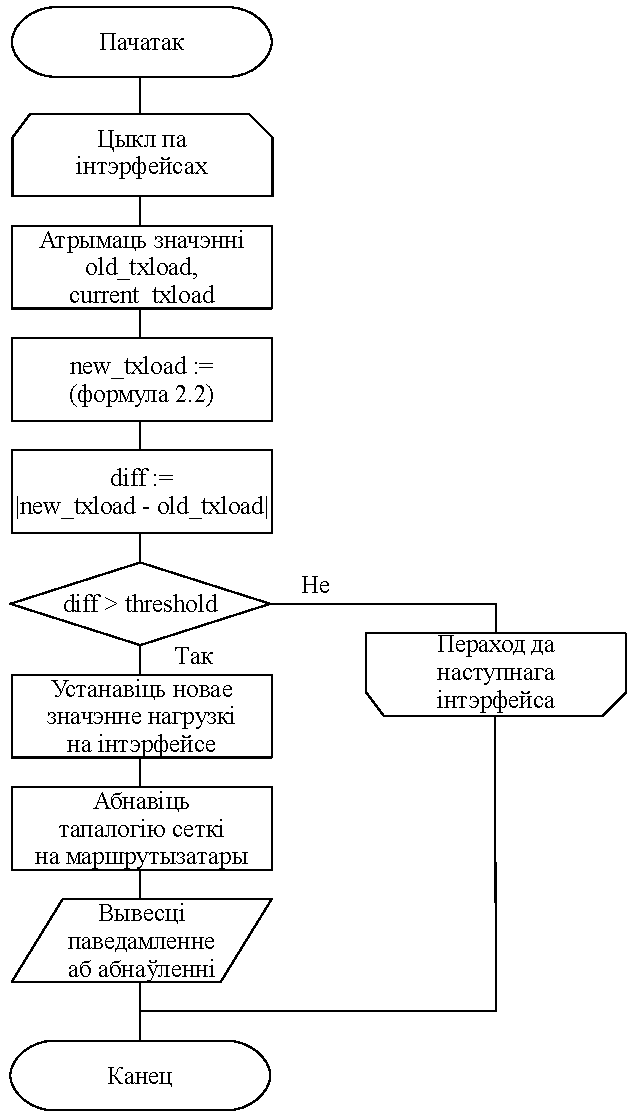
\includegraphics[width=0.55\linewidth]{block-schema.pdf}
    \caption{Блок-схема алгарытму пераразліку нагрузкі}
    \label{img: block-schema}
\end{figure}

\subsection{Механізм збору інфармацыі з сеткавага вузла}

Разглядаемы вышэй алгарытм прапануецца выкарыстоўваць у рамках гібрыднай
рэалізацыі праграмна-вызначаных сетак.

Пры рэалізацыі дадзенага метада на практыцы выкарыстоўваліся:
\begin{enumerate}
    \item Сеткавае абсталяванне Cisco Systems Inc.;
    \item Restconf протокол для збору інфармацыі.
\end{enumerate}

RESTCONF аб'ядноўвае прастату HTTP з прадказальнасцю і магчымасцямі аўтаматызацыі кіраванымі схемамі API. Ведаючы модулі YANG, якія выкарыстоўваeцца сервер, кліент можа вывесці URL ўсіх рэсурсаў кіравання, а таксама прыдатную структуру ўсіх запытаў і водгукаў RESTCONF.

RESTCONF выкарыстоўвае бібліятэку YANG для прадастаўлення кліентам магчымасці знайсці інфармацыю у адпаведнасці з модулем YANG на сeрвэры, калі кліент хоча скарыстацца ёй.

Ідэнтыфікатары URI для залежных ад мадэлі даных аперацый RPC і змесціва сховішчаў прадказальныя на аснове азначэнняў у модулі YANG.

RESTCONF працуе з канцэптуальным сховішчам даных, вызначаным на мове мадэлявання YANG. Сервер пералічвае ўсе падтрымоўваныя модулі YANG з выкарыстаннем модуля ietf-yang-library. Сервер павінен рэалізаваць модуль ietf-yang-library, які павінен паказваць усе выкарыстоўваныя серверам модулі YANG ў спісе modules-state/module. Змесціва канцэптуальнага сховішчы даных, залежныя ад мадэлі аперацыі RPC і апавяшчэння аб падзеях таксама паказваюцца гэтым наборам модуляў YANG.

Класіфікацыя даных якія адносяцца ці якія не адносяцца да канфігурацый выводзіцца з аператара YANG config. Паводзіны, звязанае з парадкаваннем даных, вызначаецца аператарам YANG ordered-by. Даныя, якія не адносяцца да канфігурацыі, называюць таксама данымі стану.

Мадэль рэдагавання сховішчы даных у RESTCONF простая і прамалінейная, падобна паводзінам магчымасці :writable-running ў NETCONF. Кожнае рэдагаванне RESTCONF рэсурсу даных у рэсурсе сховішчы актывіруецца пасля паспяховага завяршэння рэдагавання.

\subsection{Рэалізацыя механізму пераразліку нагрузкі}

Праграма, якая рэалізуе вышэй апісаны алгарытм уліку нагрузкі, напісана
на аб'ектна-арыентаванай мове праграмавання Python. Выбар у якасці мовы праграмавання
Python абумоўлены яго шматплатформеннасцю, а таксама вялікай колькасцю модуляў і бібліятэк, якія пашыраюць базавы функцыянал.

Праграма складаецца з 3 асноўных частак:
\begin{enumerate}
    \item Recalculation --- клас, які адказвае за працэс маніторынгу параметраў маршрутызатара і прыняцця рашэння аб
    пераразліку тапалогіі сеткі;
    \item Router --- клас, які ўяўляе сабой апісанне маршртузатара, і рэалізуе
    метады збору і перадачы інфармацыі на маршрутызатар;
    \item Interface --- клас, які ўяўляе сабой апісанне інтэрфейса маршрутызатара,
    і рэалізуе метады збору інфармацыі з дадзенага інтэрфейса.
\end{enumerate}

На малюнку \ref{uml: Class Diagram} прадстаўлена дыяграма класаў.

\clearpage

\begin{figure}[ht!]
    \centering
    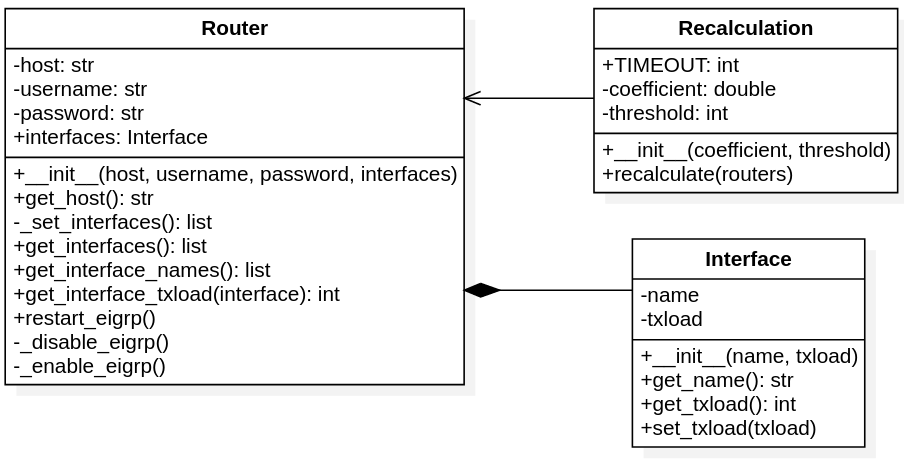
\includegraphics[width=\textwidth]{class_diagram.png}
    \caption{Дыяграма класаў праграмы пераліку нагрузкі}
    \label{uml: Class Diagram}
\end{figure}

\vspace{-\baselineskip}

\subsubsection{Апісанне класса Interface.}

Дадзены клас змяшчае ўсю неабходную інфармацыю пра інтэрфейс маршрутызатара і
рэалізуе метады для работы з ім.

Атрыбуты класа:
\begin{enumerate}
    \item name --- імя інтэрфейса на маршрутызатары (напрыклад, GigabitEthernet1);
    \item txload --- значэнне нагрузкі перадачы на інтэрфейсе.
\end{enumerate}

Метады класа:
\begin{enumerate}
    \item get\_name() --- вяртае імя інтэрфейса;
    \item get\_txload() --- вяртае значэнне нагрузкі перадачы на інтэрфейсе;
    \item set\_txload(txload) --- выстаўляе значэнне нагрузкі перадачы на інтэрфейсе
    роўным txload.
\end{enumerate}

У лістынгу \ref{lst: interface} прадстаўлены зыходны код Interface класа.

\lstinputlisting[caption={Зыходны код Interface класа},%
                            label={lst: interface},%
                            language=Python]{interface.py}

\vspace{-\baselineskip}

\subsubsection{Апісанне класа Router.}

Дадзены клас змяшчае ўсю неабходную інфармацыю пра маршрутызатар і рэалізуе
метады для работы з ім.

Атрыбуты класа:
\begin{enumerate}
    \item host --- IP-адрас маршрутызатара, на які будзе ажыццяўляцца падключэнне кантролерам;
    \item username --- імя карыстальніка для аўтэнтыфікацыі і аўтарызацыі;
    \item password --- пароль карыстальніка для аўтэнтыфікацыі і аўтарызацыі;
    \item interfaces --- спіс усіх інтэрфейсаў на маршрутызатары.
\end{enumerate}

Метады класа:
\begin{enumerate}
    \item get\_host() --- вяртае IP-адрас маршрутызатара;
    \item \_set\_interfaces() --- збірае і ўстанаўлівае інфармацыю пра інтэрфейсы на маршрутызатары;
    \item get\_interfaces() --- вяртае ўсе інтэрфейсы маршрутызатара;
    \item get\_interface\_names() --- вяртае ўсе назвы інтэрфейсаў;
    \item get\_interface\_txload(interface) --- вяртае нагрузку перадачы інтэрфейса;
    \item restart\_eigrp() --- перазагружае eigrp пратакол для пералічэння сеткавай тапалогіі;
    \item \_disable\_eigrp() --- адключае eigrp пратакол;
    \item \_enable\_eigrp() --- уключае eigrp пратакол.
\end{enumerate}

У лістынгу \ref{lst: router} прадстаўлены зыходны код Router класа.

\lstinputlisting[caption={Зыходны код Router класа},%
                            label={lst: router},%
                            language=Python]{router.py}

\vspace{-\baselineskip}

\subsubsection{Апісанне класа Recalculation.}

Дадзены клас рэалізуе механізм маніторынгу і прыняцця рашэння для пераразліку тапалогіі сеткі на маршрутызатары.
Клас Recalculation унаследаваны ад класа Thread (модуль threading) для рэалізацыі паралельнай работы кантролера для
некалькіх маршрутызатараў: для кожнага маршрутызатара выкарыстоўваецца асобны паток.

Атрыбуты класа:
\begin{enumerate}
    \item TIMEOUT --- прамежак часу (у секундах) праз які запрашваецца значэнне нагрузкі з інтэрфейсаў маршрутызатара;
    \item coefficient --- значэнне каэфіцыента $\alpha$;
    \item threshold --- парог рознасці паміж новай і старой нагрузкай, пры
    перавышэнні якога адпраўляецца каманда на перабудову сеткавай тапалогіі.
\end{enumerate}

Метад класа:
\begin{enumerate}
    \item run() --- перазапіс метада класа Thread для паралельнага выконвання праграмы. Выконвае маніторынг і пералік нагрузкі для маршрутызатараў, інфармацыя пра якіх была перададзена ў метад.
\end{enumerate}

У лістынгу \ref{lst: recalculation} прадстаўлены зыходны код Recalculation класа.

\lstinputlisting[caption={Зыходны код Recalculation класа},%
                            label={lst: recalculation},%
                            language=Python]{recalculation.py}

У лістынгу  \ref{lst: main} прадстаўлены прыклад запуску праграмы для адсочвання
нагрузкі і пералічэння сеткавай тапалогіі для 1 маршрутызатара.

\lstinputlisting[caption={Зыходны код галоўнай праграмы для 1 маршрутызатара},%
                            label={lst: main},%
                            language=Python]{main.py}

